\documentclass[titlepage]{article}
\usepackage[utf8]{inputenc}
\usepackage{amsmath, amssymb, amsthm}
\usepackage{algorithmicx}
\usepackage{graphicx}
\usepackage{subcaption}
\usepackage{listings}
\usepackage{color}
\usepackage{mdframed}
\usepackage{float}
\usepackage{booktabs}
\usepackage{mathtools}

\newcommand{\diag}{\operatorname{diag}}

\definecolor{dkgreen}{rgb}{0,0.6,0}
\definecolor{gray}{rgb}{0.5,0.5,0.5}
\definecolor{mauve}{rgb}{0.58,0,0.82}

\lstset{frame=single,
	language=matlab,
	aboveskip=3mm,
	belowskip=3mm,
	showstringspaces=false,
	columns=flexible,
	basicstyle={\small\ttfamily},
	numbers=none,
	numberstyle=\tiny\color{gray},
	keywordstyle=\color{blue},
	commentstyle=\color{dkgreen},
	stringstyle=\color{mauve},
	breaklines=true,
	breakatwhitespace=true,
	tabsize=3
}

\setlength{\parindent}{0pt}

\title{AAE 50700: Principles of Dynamics\\ Problem Set 3 Report}
\author{Dylan Ashby}
\date{\today}

\begin{document}

\maketitle

\section*{(3.1) Constraints, Virtual Work, and D'Alembert's Principle}

Consider a rigid bus $B$ with a rigid solar array attached via a hinge. Fig. \ref{fig:setup} shows a top-down view of the satellite. A rigid, thin solar-array paddle $A$ is connected to $B$ via a friction-less hinge $H$ on $B$. Both Problem Set 3 and Problem Set 4 will focus on the planar motion of the satellite in the inertial frame $\mathcal{N}"\{\hat{\boldsymbol{n}}_1,\hat{\boldsymbol{n}}_1\}$.\\

Relevant quantities and parameters are defined as follows:
\begin{itemize}
	\item \textbf{Bus}: $C_B$, $m_B$, and $J_{C_B}$ denote the bus center of mass (CoM), mass, and moment of inertia about $C_B$, respectively. The bus is a cube of side length 2$l$ and of uniform density.
	\item \textbf{Array:} $C_A$, $m_A$, and $J_{C_A}$ denote the array CoM, mass, and moment of inertia about $C_A$ respectively. The $H-C_A$ distance is $d$.
\end{itemize}

The positions of $C_B$ and $C_A$ measured from the origin are given by:
\begin{equation}
	\boldsymbol{r}_{C_B}(t)=x_{C_B}(t)\hat{\boldsymbol{n}}_1+y_{C_B}(t)\hat{\boldsymbol{n}}_2
\end{equation}

\begin{figure}[H]
	\centering
	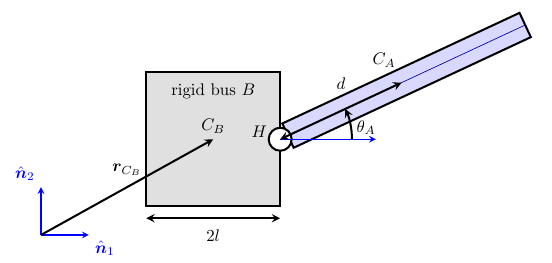
\includegraphics[width=0.85\textwidth]{setup.png}
	\caption{Top-down view of satellite bus $B$ and solar array $A$, which are both assumed rigid. Both Problem Set 3 and Problem Set 4 consider this system.}
	\label{fig:setup}
\end{figure}

\newpage

\section*{(4.1) Lagrange's Equations}

\subsection*{(a): Given}
Starting from Lagrangian form of D'Alembert's principle.\\

\textbf{Find:}\\
Derive the Lagrange's equations for non-conservative systems with minimal coordinates $\boldsymbol{q}$.\\

\textbf{Analysis/Conclusions:}\\
The Lagrangian form of D'Alembert's principle for minimal coordinates is written as:
\begin{equation}
	\sum_{i=1}^{N}m_i\ddot{\boldsymbol{r}}_i\cdot\frac{\partial\boldsymbol{r}_i}{\partial q_j}=Q_j\,\forall j
	\label{eq:dalembert}
\end{equation}
With mass $m_i$, position $\boldsymbol{r}_i$, and $N$ representing the number of particles in a model.\\

The generalized force term $Q_j$ can be represented by:
\begin{equation}
	Q_j=\sum_{i=1}^{N}\boldsymbol{F}_i\cdot\frac{\partial\boldsymbol{r}_i}{\partial q_j}
	\label{eq:genforce}
\end{equation}

The core of Lagrange's idea was to use the partial derivative of kinetic energy $T$ with respect to ($q_j$,$\dot{q}_j$) with the above D'Alembert's equations. Recall the general expression for kinetic energy is:
\begin{equation}
	T=\frac{1}{2}\sum_{i=1}^{N}m_i\dot{\boldsymbol{r}}_i\cdot\dot{\boldsymbol{r}}_i
\end{equation}

Then we find the two derivatives as:
\begin{equation}
	\begin{split}
		\frac{\partial T}{\partial q_j}&=\frac{\partial}{\partial q_j}\left(\frac{1}{2}\sum_{i=1}^{N}m_i\dot{\boldsymbol{r}}_i\cdot\dot{\boldsymbol{r}}_i\right)=\sum_{i=1}^{N}m_i\dot{\boldsymbol{r}}_i\cdot\frac{\partial\dot{\boldsymbol{r}}_i}{\partial q_j} \\
		\frac{\partial T}{\partial\dot{q}_j}&=\frac{\partial}{\partial\dot{q}_j}\left(\frac{1}{2}\sum_{i=1}^{N}m_i\dot{\boldsymbol{r}}_i\cdot\dot{\boldsymbol{r}}_i\right)=\sum_{i=1}^{N}m_i\dot{\boldsymbol{r}}_i\cdot\frac{\partial\dot{\boldsymbol{r}}_i}{\partial\dot{q}_j}
	\end{split}
	\label{eq:energyderivative}
\end{equation}

Then, since $\boldsymbol{r}_i(\boldsymbol{q},t)$ is not a function of the derivatives of $q_j$, then the cancellation of dots identity applies where:
\begin{equation}
	\frac{\partial\dot{\boldsymbol{r}}_i}{\partial\dot{q}_j}=\frac{\partial\boldsymbol{r}_i}{\partial q_j}
\end{equation}

Using this identity, Eq.~(\ref{eq:genforce}) can be rewritten as:
\begin{equation}
	Q_j=\sum_{i=1}^{N}\boldsymbol{F}_i\cdot\frac{\partial\boldsymbol{r}_i}{\partial q_j}=\sum_{i=1}^{N}\boldsymbol{F}_i\cdot\frac{\partial\dot{\boldsymbol{r}}_i}{\partial\dot{q}_j}
	\label{eq:genforcedot}
\end{equation}

Then we can take the time derivative found in the second equation in Eq.~(\ref{eq:energyderivative}). Note the application of the cancellation of dots identity on line three:
\begin{equation}
	\begin{split}
		\frac{d}{dt}\left(\frac{\partial T}{\partial\dot{q}_j}\right)&=\frac{d}{dt}\left(\sum_{i=1}^{N}m_i\dot{\boldsymbol{r}}_i\cdot\frac{\partial\dot{\boldsymbol{r}}_i}{\partial\dot{q}_j}\right) \\
		&=\sum_{i=1}^{N}m_i\frac{d\dot{\boldsymbol{r}}_i}{dt}\cdot\frac{\partial\dot{\boldsymbol{r}}_i}{\partial\dot{q}_j}+\sum_{i=1}^{N}m_i\dot{\boldsymbol{r}}_i\cdot\frac{d}{dt}\frac{\partial\dot{\boldsymbol{r}}_i}{\partial\dot{q}_j} \\
		&=\sum_{i=1}^{N}m_i\frac{d\dot{\boldsymbol{r}}_i}{dt}\cdot\frac{\partial\dot{\boldsymbol{r}}_i}{\partial\dot{q}_j}+\sum_{i=1}^{N}m_i\dot{\boldsymbol{r}}_i\cdot\frac{d}{dt}\frac{\partial\boldsymbol{r}_i}{\partial q_j} \\
		&=\sum_{i=1}^{N}m_i\ddot{\boldsymbol{r}}_i\cdot\frac{\partial\dot{\boldsymbol{r}}_i}{\partial\dot{q}_j}+\sum_{i=1}^{N}m_i\dot{\boldsymbol{r}}_i\cdot\frac{\partial\dot{\boldsymbol{r}}_i}{\partial q_j}
	\end{split}
	\label{eq:lagrangepart1}
\end{equation}

Then we notice two things: first, since Eq.~(\ref{eq:dalembert}) gives $\sum_{i=1}^{N}m_i\ddot{\boldsymbol{r}}_i\cdot\frac{\partial\boldsymbol{r}_i}{\partial q_j}=Q_j$, we see that the left half of Eq.~(\ref{eq:lagrangepart1}), is equal to the term that came from cancellation of dots on $Q_j$ in Eq.~(\ref{eq:genforcedot}). Second, we see that the right half of  Eq.~(\ref{eq:lagrangepart1}) is equal to the first equation from the derivatives in Eq.~(\ref{eq:energyderivative}). In other words:
\begin{equation}
	Q_j=\sum_{i=1}^{N}m_i\ddot{\boldsymbol{r}}_i\cdot\frac{\partial\dot{\boldsymbol{r}}_i}{\partial\dot{q}_j},\qquad \frac{\partial T}{\partial q_j}=\sum_{i=1}^{N}m_i\dot{\boldsymbol{r}}_i\cdot\frac{\partial\dot{\boldsymbol{r}}_i}{\partial q_j}
\end{equation}
Which then means the last line of Eq.~(\ref{eq:lagrangepart1}) substitutes to:
\begin{equation}
	\frac{d}{dt}\left(\frac{\partial T}{\partial\dot{q}_j}\right)=Q_j+ \frac{\partial T}{\partial q_j}
\end{equation}
\begin{mdframed}[linewidth=1pt, innertopmargin=10pt, innerbottommargin=10pt]
	And trivially rewrites to the fundamental form of Lagrange's equations for non-conservative systems with minimal coordinates $\boldsymbol{q}$:
	\begin{equation}
		Q_j=\frac{d}{dt}\left(\frac{\partial T}{\partial\dot{q}_j}\right)-\frac{\partial T}{\partial q_j}\,\forall j
	\end{equation}
\end{mdframed}

\newpage

\subsection*{(b): Given}
Consider array $A$ attached to the bus $B$ that is moving in the same manner as in Eq.~(\ref{eq:perscribed}) (translational motion only).
\begin{equation}
	\boldsymbol{r}_{C_B}(t)=X_B\cos\Omega t\hat{\boldsymbol{n}}_1,\quad\boldsymbol{r}_H(t)=\boldsymbol{r}_{C_B}(t)+l\hat{\boldsymbol{n}}_1
	\label{eq:perscribed}
\end{equation}
The array has a torsional spring at $H$ with potential:
\begin{equation}
	V_H(\theta_A)=\frac{k_H}{2}\left(\theta_A-\theta_0\right)^2
	\label{eq:springpotential}
\end{equation}

\subsubsection*{(b.1): Find}
Derive the expression of $\boldsymbol{r}_{C_A}$ in terms of $\boldsymbol{r}_H$, $d$, $\theta_A$, $\hat{\boldsymbol{n}}_1$, $\hat{\boldsymbol{n}}_2$.\\

\textbf{Analysis/Conclusions:}\\
Recall from problem set 3, we can write the unit vector pointing from the hinge $H$ to the array CoM $C_A$ using:
\begin{equation}
	\hat{\boldsymbol{e}}_A=\cos\theta_A\hat{\boldsymbol{n}}_1+\sin\theta_A\hat{\boldsymbol{n}}_2
\end{equation}

Then we can define the position of $\boldsymbol{r}_{C_A}$ as a sum of the position of the hinge $\boldsymbol{r}_H$ and the vector $\hat{\boldsymbol{e}}_A$ scaled by $d$. This is because $\boldsymbol{r}_H$ offsets the coordinates to the hinge position, $\hat{\boldsymbol{e}}_A$ points towards the array, and $d$ scales that unit vector to the distance of the array CoM from the hinge. This is written as:
\begin{equation}
	\boldsymbol{r}_{C_A}=\boldsymbol{r}_H+d\hat{\boldsymbol{e}}_A
\end{equation}
\begin{mdframed}[linewidth=1pt, innertopmargin=10pt, innerbottommargin=10pt]
	Then substituting this in with the given definition of $\hat{\boldsymbol{e}}_A$, we get the equation for $\boldsymbol{r}_{C_A}$:
	\begin{equation}
		\boldsymbol{r}_{C_A}=\boldsymbol{r}_H+d\left(\cos\theta_A\hat{\boldsymbol{n}}_1+\sin\theta_A\hat{\boldsymbol{n}}_2\right)
	\end{equation}
\end{mdframed}

\newpage

\subsubsection*{(b.2): Find}
Calculate the kinetic energy:
\begin{equation}
	T_A=\frac{m_A}{2}\dot{\boldsymbol{r}}_{C_A}\cdot\dot{\boldsymbol{r}}_{C_A}+\frac{J_{C_A}}{2}\dot{\theta}_A^2
	\label{eq:bkinetic}
\end{equation}
and form $L_A(\theta_A,\dot{\theta}_A,t)=T_A-V_H$.\\

\textbf{Analysis/Conclusions:}\\
To find the kinetic energy from the given equations, we must first find the first derivative of $\boldsymbol{r}_{C_A}$:
\begin{equation}
	\begin{split}
		\dot{\boldsymbol{r}}_{C_A}&=\frac{d}{dt}\left(\boldsymbol{r}_H+d\left(\cos\theta_A\hat{\boldsymbol{n}}_1+\sin\theta_A\hat{\boldsymbol{n}}_2\right)\right) \\
		&=\frac{d\boldsymbol{r}_H}{dt}+d\left(\frac{d}{d\theta_A}\cos\theta_A\frac{d\theta_A}{dt}\hat{\boldsymbol{n}}_1+\frac{d}{d\theta_A}\sin\theta_A\frac{d\theta_A}{dt}\hat{\boldsymbol{n}}_2\right) \\
		&=\dot{\boldsymbol{r}}_H-d\sin\theta_A\,\dot{\theta}_A\hat{\boldsymbol{n}}_1+d\cos\theta_A\,\dot{\theta}_A\hat{\boldsymbol{n}}_2 \\
	\end{split}
		\label{eq:rcadot}
\end{equation}

And the first derivative of $\boldsymbol{r}_H$:
\begin{equation}
	\begin{split}
		\dot{\boldsymbol{r}}_H&=\frac{d}{dt}\left(\boldsymbol{r}_{C_B}+l\hat{\boldsymbol{n}}_1\right) \\
		&=\frac{d}{dt}\left(X_B\cos\Omega t\hat{\boldsymbol{n}}_1+l\hat{\boldsymbol{n}}_1\right) \\
		&=X_B\frac{d}{dt}\cos\Omega t\,\hat{\boldsymbol{n}}_1+\frac{d}{dt}l\hat{\boldsymbol{n}}_1 \\
		&=-X_B\Omega\sin\Omega t\,\hat{\boldsymbol{n}}_1
	\end{split}
\end{equation}

Then compute the dot product in Eq.~(\ref{eq:bkinetic}) by substituting in the two derivatives:
\begin{equation}
	\begin{split}
		\dot{\boldsymbol{r}}_{C_A}\cdot\dot{\boldsymbol{r}}_{C_A}&=\left(\dot{\boldsymbol{r}}_H-d\sin\theta_A\,\dot{\theta}_A\hat{\boldsymbol{n}}_1+d\cos\theta_A\,\dot{\theta}_A\hat{\boldsymbol{n}}_2\right)\cdot\left(\dot{\boldsymbol{r}}_H-d\sin\theta_A\,\dot{\theta}_A\hat{\boldsymbol{n}}_1+d\cos\theta_A\,\dot{\theta}_A\hat{\boldsymbol{n}}_2\right) \\
		&=\left(-X_B\Omega\sin\Omega t-d\sin\theta_A\,\dot{\theta}_A\right)^2+\left(d\cos\theta_A\,\dot{\theta}_A\right)^2 \\
		&=X_B^2\Omega^2\sin^2\Omega t+2X_B\Omega d\,\dot{\theta}_A\sin\Omega t\sin\theta_A+d^2\sin^2\theta_A\,\dot{\theta}_A^2+d^2\cos^2\theta_A\,\dot{\theta}_A^2 \\
		&=X_B^2\Omega^2\sin^2\Omega t+2X_B\Omega d\,\dot{\theta}_A\sin\Omega t\sin\theta_A+\left(\sin^2\theta_A+\cos^2\theta_A\right)d^2\dot{\theta}_A^2 \\
		&=X_B^2\Omega^2\sin^2\Omega t+2X_B\Omega d\,\dot{\theta}_A\sin\Omega t\sin\theta_A+d^2\dot{\theta}_A^2 \\
	\end{split}
\end{equation}

Then we can find the kinetic energy $T_A$:
\begin{equation}
	\begin{split}
		T_A&=\frac{m_A}{2}\dot{\boldsymbol{r}}_{C_A}\cdot\dot{\boldsymbol{r}}_{C_A}+\frac{J_{C_A}}{2}\dot{\theta}_A^2 \\
		&=\frac{m_A}{2}\left(X_B^2\Omega^2\sin^2\Omega t+2X_B\Omega d\,\dot{\theta}_A\sin\Omega t\sin\theta_A+d^2\dot{\theta}_A^2\right)+\frac{J_{C_A}}{2}\dot{\theta}_A^2 \\
		&=\frac{m_A}{2}\left(X_B^2\Omega^2\sin^2\Omega t+2X_B\Omega d\,\dot{\theta}_A\sin\Omega t\sin\theta_A\right)+\frac{m_Ad^2+J_{C_A}}{2}\dot{\theta}_A^2 
	\end{split}
\end{equation}

\begin{mdframed}[linewidth=1pt, innertopmargin=10pt, innerbottommargin=10pt]
	So, the scalar kinetic energy equation can be written as:
	\begin{equation}
		T_A=\frac{m_A}{2}X_B^2\Omega^2\sin^2\Omega t+m_AX_B\Omega d\,\dot{\theta}_A\sin\Omega t\sin\theta_A+\frac{m_Ad^2+J_{C_A}}{2}\dot{\theta}_A^2
		\label{eq:bkineticsolved}
	\end{equation}
	Then, finding the Lagrangian $L_A(\theta_A,\dot{\theta}_A,t)$ is as simple as substituting Eq.~(\ref{eq:bkineticsolved}) and Eq.~(\ref{eq:springpotential}) into the following:
	\begin{equation}
		\begin{split}
			L_A&=T_A-V_H \\
			&=\frac{m_A}{2}X_B^2\Omega^2\sin^2\Omega t+m_AX_B\Omega d\,\dot{\theta}_A\sin\Omega t\sin\theta_A\\ &\quad+\frac{m_Ad^2+J_{C_A}}{2}\dot{\theta}_A^2-\frac{k_H}{2}\left(\theta_A-\theta_0\right)^2
		\end{split}
		\label{eq:blagrangian}
	\end{equation}
\end{mdframed}

\subsubsection*{(b.3): Find}
Verify the cancellation-of-dots identity $\frac{\partial\dot{\boldsymbol{r}}_{C_A}}{\partial\dot{\theta}_A}=\frac{\partial\boldsymbol{r}_{C_A}}{\partial\theta_A}$.\\

\textbf{Analysis/Conclusions:}\\
To verify the identity, first we compute $\frac{\partial\boldsymbol{r}_{C_A}}{\partial\theta_A}$ using the equation found in part (b.1). Recall that $\boldsymbol{r}_H$ is not a function of $\theta_A$:
\begin{equation}
	\begin{split}
		\frac{\partial\boldsymbol{r}_{C_A}}{\partial\theta_A}&=\frac{\partial}{\partial\theta_A}\left(\boldsymbol{r}_H+d\left(\cos\theta_A\hat{\boldsymbol{n}}_1+\sin\theta_A\hat{\boldsymbol{n}}_2\right)\right) \\
		&=\frac{\partial\boldsymbol{r}_H}{\partial\theta_A}+d\left(\frac{\partial}{\partial\theta_A}\cos\theta_A\,\hat{\boldsymbol{n}}_1+\frac{\partial}{\partial\theta_A}\sin\theta_A\,\hat{\boldsymbol{n}}_2\right) \\
		&=d\left(-\sin\theta_A\,\hat{\boldsymbol{n}}_1+\cos\theta_A\,\hat{\boldsymbol{n}}_2\right) \\
	\end{split}
\end{equation}

Then do the same for $\frac{\partial\dot{\boldsymbol{r}}_{C_A}}{\partial\dot{\theta}_A}$ using the derivative found in Eq.~(\ref{eq:rcadot}). $\dot{\boldsymbol{r}}_H$ is not a function of $\dot{\theta}_A$:
\begin{equation}
	\begin{split}
		\frac{\partial\dot{\boldsymbol{r}}_{C_A}}{\partial\dot{\theta}_A}&=\frac{\partial}{\partial\dot{\theta}_A}\left(\dot{\boldsymbol{r}}_H-d\sin\theta_A\,\dot{\theta}_A\hat{\boldsymbol{n}}_1+d\cos\theta_A\,\dot{\theta}_A\hat{\boldsymbol{n}}_2\right) \\
		&= \frac{\partial\dot{\boldsymbol{r}}_H}{\partial\dot{\theta}_A}+d\left(-\sin\theta_A\,\frac{\partial\dot{\theta}_A}{\partial\dot{\theta}_A}\hat{\boldsymbol{n}}_1+\cos\theta_A\,\frac{\partial\dot{\theta}_A}{\partial\dot{\theta}_A}\hat{\boldsymbol{n}}_2\right) \\
		&=d\left(-\sin\theta_A\,\hat{\boldsymbol{n}}_1+\cos\theta_A\,\hat{\boldsymbol{n}}_2\right) \\
	\end{split}
\end{equation}

\begin{mdframed}[linewidth=1pt, innertopmargin=10pt, innerbottommargin=10pt]
	Thus we see that the cancellation-of-dots identity is verified:
	\begin{equation}
		\frac{\partial\boldsymbol{r}_{C_A}}{\partial\theta_A}=d\left(-\sin\theta_A\,\hat{\boldsymbol{n}}_1+\cos\theta_A\,\hat{\boldsymbol{n}}_2\right)=\frac{\partial\dot{\boldsymbol{r}}_{C_A}}{\partial\dot{\theta}_A}
	\end{equation}
\end{mdframed}

\subsubsection*{(b.4): Find}
Derive the Lagrange equation for $\theta_A$.\\

\textbf{Analysis/Conclusions:}\\
We can find the Lagrange equation through the standard form of Lagrange's equation for conservative systems:
\begin{equation}
	\frac{d}{dt}\left(\frac{\partial L}{\partial\dot{q}_i}\right)-\frac{\partial L}{\partial q_i}=0,\quad\forall i
	\label{eq:lagrangegeneral}
\end{equation}

Let us identify that in this context there is only one degree of freedom, which is $\theta_A$. Since $\boldsymbol{q}$ is a minimal set, there is only one generalized coordinate $q_1=\theta_A$.\\

This means Eq.~(\ref{eq:lagrangegeneral}) rewrites to:
\begin{equation}
	\frac{d}{dt}\left(\frac{\partial L_A}{\partial\dot{\theta}_A}\right)-\frac{\partial L_A}{\partial\theta_A}=0
\end{equation}

Then first we find $\frac{\partial L_A}{\partial\theta_A}$ using Eq.~(\ref{eq:blagrangian}):
\begin{equation}
	\begin{split}
		\frac{\partial L_A}{\partial\theta_A}&=\frac{\partial}{\partial\theta_A}\left(\frac{m_A}{2}X_B^2\Omega^2\sin^2\Omega t+m_AX_B\Omega d\,\dot{\theta}_A\sin\Omega t\sin\theta_A\right. \\
		&\left.\qquad+\frac{m_Ad^2+J_{C_A}}{2}\dot{\theta}_A^2-\frac{k_H}{2}\left(\theta_A-\theta_0\right)^2\right) \\
		&=\frac{\partial}{\partial\theta_A}\left(\frac{m_A}{2}X_B^2\Omega^2\sin^2\Omega t\right)+\frac{\partial}{\partial\theta_A}\left(m_AX_B\Omega d\,\dot{\theta}_A\sin\Omega t\sin\theta_A\right) \\
		&\qquad+\frac{\partial}{\partial\theta_A}\left(\frac{m_Ad^2+J_{C_A}}{2}\dot{\theta}_A^2\right)-\frac{\partial}{\partial\theta_A}\left(\frac{k_H}{2}\left(\theta_A-\theta_0\right)^2\right) \\
		&=0+m_AX_B\Omega d\,\dot{\theta}_A\sin\Omega t\frac{\partial}{\partial\theta_A}\left(\sin\theta_A\right)+0-\frac{k_H}{2}\frac{\partial}{\partial\theta_A}\left(\theta_A-\theta_0\right)^2 \\
		&=m_AX_B\Omega d\,\dot{\theta}_A\sin\Omega t\frac{\partial}{\partial\theta_A}\left(\sin\theta_A\right)-\frac{k_H}{2}\left(\frac{\partial\theta_A^2}{\partial\theta_A}-2\frac{\partial\theta_A}{\partial\theta_A}\theta_0+\frac{\partial\theta_0^2}{\partial\theta_A}\right) \\
		&=m_AX_B\Omega d\,\dot{\theta}_A\sin\Omega t\,\cos\theta_A-\frac{k_H}{2}\left(2\theta_A-2(1)\theta_0+0\right) \\
		&=m_AX_B\Omega d\,\dot{\theta}_A\sin\Omega t\,\cos\theta_A-k_H\left(\theta_A-\theta_0\right) \\
	\end{split}
\end{equation}

\newpage

Then we find $\frac{\partial L_A}{\partial\dot{\theta}_A}$ using Eq.~(\ref{eq:blagrangian}) also:
\begin{equation}
	\begin{split}
		\frac{\partial L_A}{\partial\dot{\theta}_A}&=\frac{\partial}{\partial\dot{\theta}_A}\left(\frac{m_A}{2}X_B^2\Omega^2\sin^2\Omega t+m_AX_B\Omega d\,\dot{\theta}_A\sin\Omega t\sin\theta_A\right. \\
		&\left.\qquad+\frac{m_Ad^2+J_{C_A}}{2}\dot{\theta}_A^2-\frac{k_H}{2}\left(\theta_A-\theta_0\right)^2\right) \\
		&=\frac{\partial}{\partial\dot{\theta}_A}\left(\frac{m_A}{2}X_B^2\Omega^2\sin^2\Omega t\right)+\frac{\partial}{\partial\dot{\theta}_A}\left(m_AX_B\Omega d\,\dot{\theta}_A\sin\Omega t\sin\theta_A\right) \\
		&\qquad+\frac{\partial}{\partial\dot{\theta}_A}\left(\frac{m_Ad^2+J_{C_A}}{2}\dot{\theta}_A^2\right)-\frac{\partial}{\partial\dot{\theta}_A}\left(\frac{k_H}{2}\left(\theta_A-\theta_0\right)^2\right) \\
		&=0+m_AX_B\Omega d\frac{\partial\dot{\theta}_A}{\partial\dot{\theta}_A}\sin\Omega t\sin\theta_A+\frac{m_Ad^2+J_{C_A}}{2}\frac{\partial\dot{\theta}_A^2}{\partial\dot{\theta}_A}-0 \\
		&=m_AX_B\Omega d\sin\Omega t\,\sin\theta_A+\left(m_Ad^2+J_{C_A}\right)\dot{\theta}_A \\
	\end{split}
\end{equation}

Then we find the time derivative $\frac{d}{dt}\left(\frac{\partial L_A}{\partial\dot{\theta}_A}\right)$:
\begin{equation}
	\begin{split}
		\frac{d}{dt}\left(\frac{\partial L_A}{\partial\dot{\theta}_A}\right)&=\frac{d}{dt}\left(m_AX_B\Omega d\sin\Omega t\,\sin\theta_A+\left(m_Ad^2+J_{C_A}\right)\dot{\theta}_A\right) \\
		&=m_AX_B\Omega d\left(\frac{d}{dt}\sin\Omega t\right)\sin\theta_A \\
		&\qquad+m_AX_B\Omega d\sin\Omega t\left(\frac{d}{d\theta_A}\sin\theta_A\,\frac{d\theta_A}{dt}\right)+\left(m_Ad^2+J_{C_A}\right)\frac{d\dot{\theta}_A}{dt} \\
		&=m_AX_B\Omega^2d\cos\Omega t\,\sin\theta_A \\
		&\qquad+m_AX_B\Omega d\sin\Omega t\,\cos\theta_A\,\dot{\theta}_A+\left(m_Ad^2+J_{C_A}\right)\ddot{\theta}_A \\
	\end{split}
\end{equation}

With these derivatives found, we can now assemble Lagrange's equation for $\theta_A$:
\begin{equation}
	\begin{split}
		0&=\frac{d}{dt}\left(\frac{\partial L_A}{\partial\dot{\theta}_A}\right)-\frac{\partial L_A}{\partial\theta_A} \\
		&=m_AX_B\Omega^2d\cos\Omega t\,\sin\theta_A+m_AX_B\Omega d\sin\Omega t\,\cos\theta_A\,\dot{\theta}_A+\left(m_Ad^2+J_{C_A}\right)\ddot{\theta}_A \\
		&\qquad-m_AX_B\Omega d\,\sin\Omega t\,\cos\theta_A\dot{\theta}_A+k_H\left(\theta_A-\theta_0\right) \\
		&=m_AX_B\Omega^2d\cos\Omega t\,\sin\theta_A+\left(m_Ad^2+J_{C_A}\right)\ddot{\theta}_A+k_H\left(\theta_A-\theta_0\right) \\
	\end{split}
\end{equation}
Then we put it in terms of $\ddot{\theta}_A$:
\begin{equation}
	\begin{split}
		-\left(m_Ad^2+J_{C_A}\right)\ddot{\theta}_A&=m_AX_B\Omega^2d\cos\Omega t\,\sin\theta_A+k_H\left(\theta_A-\theta_0\right) \\
		\ddot{\theta}_A&=\frac{m_AX_B\Omega^2d\cos\Omega t\,\sin\theta_A+k_H\left(\theta_A-\theta_0\right) }{-\left(m_Ad^2+J_{C_A}\right)} \\
	\end{split}
\end{equation}

\begin{mdframed}[linewidth=1pt, innertopmargin=10pt, innerbottommargin=10pt]
	Which makes the Lagrange equation:
	\begin{equation}
		\ddot{\theta}_A=-\frac{m_AX_B\Omega^2d\cos\Omega t\,\sin\theta_A+k_H\left(\theta_A-\theta_0\right)}{m_Ad^2+J_{C_A}}
	\end{equation}
\end{mdframed}

\subsubsection*{(b.5): Find}
Discuss how this EOM compares to the EOM derived in problem set 3(c) with the bias torque $\tau_H$ set to zero.\\

\textbf{Analysis/Conclusions:}\\
Recall from problem set 3(c), the EOM derived was found to be:
\begin{equation}
	\ddot{\theta}_A=\frac{\tau_H-k_H(\theta_A-\theta_0)-m_AdX_B\Omega^2\cos\Omega t\sin\theta_A}{m_Ad^2+J_{C_A}}
\end{equation}
If bias torque $\tau_H$ is set to zero, it becomes:
\begin{equation}
	\begin{split}
		\ddot{\theta}_A&=\frac{0-k_H(\theta_A-\theta_0)-m_AdX_B\Omega^2\cos\Omega t\sin\theta_A}{m_Ad^2+J_{C_A}} \\
		\ddot{\theta}_A&=-\frac{m_AX_B\Omega^2d\cos\Omega t\sin\theta_A+k_H(\theta_A-\theta_0)}{m_Ad^2+J_{C_A}} \\
	\end{split}
\end{equation}

\begin{mdframed}[linewidth=1pt, innertopmargin=10pt, innerbottommargin=10pt]
	We see that if we move some terms around, when the bias torque is set to zero, the equation from problem set 3(c) is \textbf{identical} to the EOM derived in part (b.4) of this problem set. \\
	
	This is expected because both are effectively derived from D'Alembert's principle. However, in problem set 3, the equation was derived from a two particle system, whereas in this problem set the problem was derived from the scalar kinetic energy equation and spring potential energy equations. Despite the apparent differences in the methods, the exact same EOM are derived for the array angle $\theta_A$.
\end{mdframed}

\newpage

\subsection*{(c): Given}
Suppose the bus is translationally moving as given in Eq.~(\ref{eq:perscribed}) but not rotating (same as the previous problem). Now, let us add the following motor-and-damper torque to the hinge:
\begin{equation}
	\tau_H(\dot{\theta}_A,t)=\tau_{H,a}(t)-c_H\dot{\theta}_A,\quad c_H>0
\end{equation}

\subsubsection*{(c.1): Find}
Derive the force Lagrange equation for $\theta_A$.\\

\textbf{Analysis/Conclusions:}\\
We can find the Lagrange equation through the Standard form of Lagrange's equation for non-conservative systems:
\begin{equation}
	\frac{d}{dt}\left(\frac{\partial L}{\partial\dot{q}_i}\right)-\frac{\partial L}{\partial q_i}=Q_{\text{nc},i},\quad\forall i
	\label{eq:lagrangegeneralnc}
\end{equation}

Effectively, the only difference here versus the conservative version in Eq.~(\ref{eq:lagrangegeneral}) is the inclusion of the generalized force terms coming from non-conservative forces $Q_{\text{nc},i}$.\\

Just like in part (b), since this system has only one degree of freedom due to the prescribed motion, Eq.~(\ref{eq:lagrangegeneralnc}) can be written as:
\begin{equation}
	\frac{d}{dt}\left(\frac{\partial L_A}{\partial\dot{\theta}_A}\right)-\frac{\partial L_A}{\partial\theta_A}=Q_{\text{nc},\theta_A}
	\label{eq:lagrangegstandardnc}
\end{equation}
Where $L_A$ is the same Lagrangian found in part (b). This means all that's left to do is solve for the non-conservative forces $Q_{\text{nc},\theta_A}$.\\

Using the virtual work of the applied forces in generalized coordinates, as given in class:
\begin{equation}
	\delta w=\sum_{j=1}^{n}\sum_{i=1}^{N}\boldsymbol{F}_i\cdot\frac{\partial\boldsymbol{r}_i}{\partial q_j}\delta q_j=\sum_{j=1}^{n}Q_j\delta q_j
	\label{eq:virtualwork}
\end{equation}
where $N$ is the number of particles in the system and each generalized force $Q_j$ is defined as in Eq.~(\ref{eq:genforce}). However, since there is only one dimension in the defined generalized coordinates, the virtual work of the non-conservative forces simplifies to:
\begin{equation}
	\delta w_{\text{nc}}=Q_{\text{nc},\theta_A}\delta\theta_A=\tau_H\,\delta\theta_A
\end{equation}
Where $\tau_H\,\delta\theta_A$ is the virtual work of the hinge torque, since a torque does work equal to the torque multiplied by the rotation it acts through, and the bus is not rotating, so the hinge torque acts through exactly the virtual rotation of the array $\delta\theta_A$. This means the non-conservative generalized force is simply the motor-and-damper torque:
\begin{equation}
	Q_{\text{nc},\theta_A}=\tau_H(\dot{\theta}_A,t)=\tau_{H,a}(t)-c_H\dot{\theta}_A
\end{equation}

So, then we can substitute the generalized force into Eq.~(\ref{eq:lagrangegstandardnc}) using the Lagrangian derivative terms already calculated in part (b):
\begin{equation}
	\begin{split}
		Q_{\text{nc},\theta_A}&=\frac{d}{dt}\left(\frac{\partial L_A}{\partial\dot{\theta}_A}\right)-\frac{\partial L_A}{\partial\theta_A} \\
		\tau_{H,a}(t)-c_H\dot{\theta}_A&=m_AX_B\Omega^2d\cos\Omega t\,\sin\theta_A+m_AX_B\Omega d\sin\Omega t\,\cos\theta_A\,\dot{\theta}_A \\
		&+\left(m_Ad^2+J_{C_A}\right)\ddot{\theta}_A-m_AX_B\Omega d\,\sin\Omega t\,\cos\theta_A\dot{\theta}_A+k_H\left(\theta_A-\theta_0\right) \\
		&=m_AX_B\Omega^2d\cos\Omega t\,\sin\theta_A+\left(m_Ad^2+J_{C_A}\right)\ddot{\theta}_A+k_H\left(\theta_A-\theta_0\right) \\
	\end{split}
\end{equation}
Then we once again put it in terms of $\ddot{\theta}_A$:
\begin{equation}
	\begin{split}
		\left(m_Ad^2+J_{C_A}\right)\ddot{\theta}_A&=\tau_{H,a}(t)-c_H\dot{\theta}_A-m_AX_B\Omega^2d\cos\Omega t\,\sin\theta_A-k_H\left(\theta_A-\theta_0\right) \\
		\ddot{\theta}_A&=\frac{\tau_{H,a}(t)-c_H\dot{\theta}_A-m_AX_B\Omega^2d\cos\Omega t\,\sin\theta_A-k_H\left(\theta_A-\theta_0\right)}{m_Ad^2+J_{C_A}} \\
	\end{split}
\end{equation}

\begin{mdframed}[linewidth=1pt, innertopmargin=10pt, innerbottommargin=10pt]
	Which makes the forced Lagrange equation:
	\begin{equation}
		\ddot{\theta}_A=\frac{\tau_{H,a}(t)-c_H\dot{\theta}_A-m_AX_B\Omega^2d\cos\Omega t\,\sin\theta_A-k_H\left(\theta_A-\theta_0\right)}{m_Ad^2+J_{C_A}}
		\label{eq:forcedlagrange}
	\end{equation}
\end{mdframed}

\subsubsection*{(c.2): Find}
Consider commanding the motor at $H$ to produce a prescribed array motion $\theta_A^*(t)$ while bus $B$ follows the given translational motion Eq.~(\ref{eq:perscribed}). Derive the required motor torque $\tau_{H,a}(t)$. Identify the contributions associated with array inertia, hinge damping, the spring restoring torque, and prescribed bus acceleration.\\

\textbf{Analysis/Conclusions:}\\
To derive the required $\tau_{H,a}(t)$, simply put Eq.~(\ref{eq:forcedlagrange}) in terms of $\tau_{H,a}(t)$:
\begin{equation}
	\begin{split}
		\ddot{\theta}_A&=\frac{\tau_{H,a}(t)-c_H\dot{\theta}_A-m_AX_B\Omega^2d\cos\Omega t\,\sin\theta_A-k_H\left(\theta_A-\theta_0\right)}{m_Ad^2+J_{C_A}} \\
		\left(m_Ad^2+J_{C_A}\right)\ddot{\theta}_A&=\tau_{H,a}(t)-c_H\dot{\theta}_A-m_AX_B\Omega^2d\cos\Omega t\,\sin\theta_A-k_H\left(\theta_A-\theta_0\right) \\
		\tau_{H,a}(t)&=\left(m_Ad^2+J_{C_A}\right)\ddot{\theta}_A+c_H\dot{\theta}_A \\
		&\qquad+k_H\left(\theta_A-\theta_0\right)+m_AX_B\Omega^2d\cos\Omega t\,\sin\theta_A
	\end{split}
\end{equation}


\begin{mdframed}[linewidth=1pt, innertopmargin=10pt, innerbottommargin=10pt]
	Then replace the time-varying $\theta_A(t)$ terms with prescribed $\theta_A^*(t)$ terms to get the equation:
	\begin{equation}
		\tau_{H,a}(t)=\left(m_Ad^2+J_{C_A}\right)\ddot{\theta}_A^*+c_H\dot{\theta}_A^*+k_H\left(\theta_A^*-\theta_0\right)+m_AX_B\Omega^2d\cos\Omega t\,\sin\theta_A^*
		\label{eq:motortorque}
	\end{equation}
	
	From Eq.~(\ref{eq:motortorque}), we can identify the following terms:\\
	
	$\left(m_Ad^2+J_{C_A}\right)\ddot{\theta}_A^*$ is the contributing term for the array inertia because it is the only term that scales with the angular acceleration $\ddot{\theta}_A^*$ and that is by definition inertial torque. \\
	
	$c_H\dot{\theta}_A^*$ is the contributing term for the hinge damping because it scales directly with angular rate, and damping forces/torques always scale from the first derivative term. \\
	
	$k_H\left(\theta_A^*-\theta_0\right)$ is the contributing term for the spring restoring torque because it is scaling with the displacement of the angle $\theta_A^*$ from the reference angle $\theta_0$. This means, the further the displacement from $\theta_0$, the stronger the torque will push back towards $\theta_0$.\\
	
	$m_AX_B\Omega^2d\cos\Omega t\,\sin\theta_A^*$ is the contributing term for the prescribed bus acceleration because it is the first term of $\frac{d}{dt}\left(\frac{\partial L_A}{\partial\dot{\theta}_A}\right)$ found in part (b.4), which came from taking the time derivative of $\sin\Omega t$ in the bus velocity, giving the bus acceleration.
\end{mdframed}

\newpage

\section*{(4.2) Lagrange Multipliers for Systems with Constraints}

\subsection*{(d): Given}
Suppose the bus $B$ is inertially fixed. Use the following coordinates to describe the configuration of $A$: $\boldsymbol{q}=[x_{C_A},y_{C_A},\theta_A]^T$. The rigid hinge imposes:
\begin{equation}
	\psi_1=x_{C_A}-d\cos\theta_A=0,\quad\psi_2=y_{C_A}-d\sin\theta_A=0
\end{equation}
The torsional spring at $H$ has potential $V_H(\theta_A)=\frac{k_H}{2}(\theta_A-\theta_0)^2$. The system is under the applied force at $C_A$ and the applied torque at $H$, given as $\boldsymbol{F}_A=F_{x,A}\hat{\boldsymbol{n}}_1+F_{y,A}\hat{\boldsymbol{n}}_2$ and $\tau_{H,a}$, respectively.

\subsubsection*{(d.1): Find}
Derive the Lagrangian $L(\boldsymbol{q},\dot{\boldsymbol{q}},t)$.\\

\textbf{Analysis/Conclusions:}\\
Recall from problem (b.2) that kinetic energy is given by:
\begin{equation}
	T_A=\frac{m_A}{2}\dot{\boldsymbol{r}}_{C_A}\cdot\dot{\boldsymbol{r}}_{C_A}+\frac{J_{C_A}}{2}\dot{\theta}_A^2
\end{equation}

Since the new coordinate set now also includes Cartesian coordinates on the two planar axes $x_{C_A}$ and $y_{C_A}$, we can say that:
\begin{equation}
	\dot{\boldsymbol{r}}_{C_A}=\dot{x}_{C_A}\hat{\boldsymbol{n}}_1+\dot{y}_{C_A}\hat{\boldsymbol{n}}_2
\end{equation}
Since $\dot{\boldsymbol{r}}_{C_A}$ is just the derivative of position of the array CoM, and $x_{C_A}$ and $y_{C_A}$ are the positional components aligned with basis vectors $\hat{\boldsymbol{n}}_1$ and $\hat{\boldsymbol{n}}_2$ respectively.\\

This means we can write kinetic energy as:
\begin{equation}
	\begin{split}
		T_A&=\frac{m_A}{2}\dot{\boldsymbol{r}}_{C_A}\cdot\dot{\boldsymbol{r}}_{C_A}+\frac{J_{C_A}}{2}\dot{\theta}_A^2 \\
		&=\frac{m_A}{2}\left(\dot{x}_{C_A}\hat{\boldsymbol{n}}_1+\dot{y}_{C_A}\hat{\boldsymbol{n}}_2\right)\cdot\left(\dot{x}_{C_A}\hat{\boldsymbol{n}}_1+\dot{y}_{C_A}\hat{\boldsymbol{n}}_2\right)+\frac{J_{C_A}}{2}\dot{\theta}_A^2 \\
		&=\frac{m_A}{2}\left(\dot{x}_{C_A}^2+\dot{y}_{C_A}^2\right)+\frac{J_{C_A}}{2}\dot{\theta}_A^2 \\
	\end{split}
	\label{eq:kineticenergynonmin}
\end{equation}
Which puts kinetic energy $T_A$ in terms of generalized coordinates $\boldsymbol{q}$.\\

\newpage

\begin{mdframed}[linewidth=1pt, innertopmargin=10pt, innerbottommargin=10pt]
	Then finding the Lagrangian $L(\boldsymbol{q},\dot{\boldsymbol{q}},t)$ can be found by substituting Eq.~(\ref{eq:kineticenergynonmin}) and the potential energy equation $V_H(\theta_A)$ given by the problem into the following:
	\begin{equation}
		\begin{split}
			L&=T_A-V_H \\
			L&=\frac{m_A}{2}\left(\dot{x}_{C_A}^2+\dot{y}_{C_A}^2\right)+\frac{J_{C_A}}{2}\dot{\theta}_A^2-\frac{k_H}{2}(\theta_A-\theta_0)^2 \\
		\end{split}
	\end{equation}
\end{mdframed}

\subsubsection*{(d.2): Find}
Derive the Lagrange equations using multipliers $\lambda_{H,1}$ and $\lambda_{H,2}$.\\

\textbf{Analysis/Conclusions:}\\
Now that we are modeling constraint forces, we must assume $\boldsymbol{q}$ is now a non-minimal coordinate set. The standard form of Lagrange's equation for non-conservative systems assuming a non-minimal coordinates set expands upon Eq.~(\ref{eq:lagrangegeneralnc}):
\begin{equation}
	\frac{d}{dt}\left(\frac{\partial L}{\partial\dot{q}_i}\right)-\frac{\partial L}{\partial q_i}=Q_{\text{nc},i}+\sum_{j=1}^{m}\lambda_j\frac{\partial\psi_j}{\partial q_i},\quad i=1,...,n
\end{equation}
Where $i$ indexes the coordinates of $\boldsymbol{q}$ and $m$ represents the number of constraints indexed by $j$.\\

Since there are now three coordinates in $\boldsymbol{q}$, there are also three Lagrange equations. Below, they will be derived one at a time.\\

First for the coordinate $q_1=x_{C_A}$, the Lagrange equation can be written the following way:
\begin{equation}
	\frac{d}{dt}\left(\frac{\partial L}{\partial\dot{x}_{C_A}}\right)-\frac{\partial L}{\partial x_{C_A}}=Q_{\text{nc},x_{C_A}}+\lambda_1\frac{\partial\psi_1}{\partial x_{C_A}}+\lambda_2\frac{\partial\psi_2}{\partial x_{C_A}}
	\label{eq:xca}
\end{equation}

Evaluating $\frac{\partial L}{\partial x_{C_A}}$:
\begin{equation}
	\begin{split}
		\frac{\partial L}{\partial x_{C_A}}&=\frac{\partial}{\partial x_{C_A}}\left(\frac{m_A}{2}\left(\dot{x}_{C_A}^2+\dot{y}_{C_A}^2\right)+\frac{J_{C_A}}{2}\dot{\theta}_A^2-\frac{k_H}{2}(\theta_A-\theta_0)^2\right) \\
		&=\frac{\partial}{\partial x_{C_A}}\left(\frac{m_A}{2}\left(\dot{x}_{C_A}^2+\dot{y}_{C_A}^2\right)\right)+\frac{\partial}{\partial x_{C_A}}\left(\frac{J_{C_A}}{2}\dot{\theta}_A^2\right)-\frac{\partial}{\partial x_{C_A}}\left(\frac{k_H}{2}(\theta_A-\theta_0)^2\right) \\
		&=0+0-0=0 \\
	\end{split}
\end{equation}

Evaluating $\frac{\partial L}{\partial\dot{x}_{C_A}}$:
\begin{equation}
	\begin{split}
		\frac{\partial L}{\partial\dot{x}_{C_A}}&=\frac{\partial}{\partial\dot{x}_{C_A}}\left(\frac{m_A}{2}\left(\dot{x}_{C_A}^2+\dot{y}_{C_A}^2\right)+\frac{J_{C_A}}{2}\dot{\theta}_A^2-\frac{k_H}{2}(\theta_A-\theta_0)^2\right) \\
		&=\frac{\partial}{\partial\dot{x}_{C_A}}\left(\frac{m_A}{2}\left(\dot{x}_{C_A}^2+\dot{y}_{C_A}^2\right)\right)+\frac{\partial}{\partial\dot{x}_{C_A}}\left(\frac{J_{C_A}}{2}\dot{\theta}_A^2\right)-\frac{\partial}{\partial\dot{x}_{C_A}}\left(\frac{k_H}{2}(\theta_A-\theta_0)^2\right) \\
		&=\frac{m_A}{2}\left(\frac{\partial\dot{x}_{C_A}^2}{\partial\dot{x}_{C_A}}+\frac{\partial\dot{y}_{C_A}^2}{\partial\dot{x}_{C_A}}\right)+0-0 \\
		&=\frac{m_A}{2}\left(2\dot{x}_{C_A}+0\right)=m_A\dot{x}_{C_A} \\
	\end{split}
\end{equation}

Evaluating $\frac{d}{dt}\left(\frac{\partial L}{\partial\dot{x}_{C_A}}\right)$:
\begin{equation}
	\frac{d}{dt}\left(\frac{\partial L}{\partial\dot{x}_{C_A}}\right)=\frac{d}{dt}\left(m_A\dot{x}_{C_A}\right)=m_A\frac{d\dot{x}_{C_A}}{dt}=m_A\ddot{x}_{C_A}
\end{equation}

Evaluating $\frac{\partial\psi_1}{\partial x_{C_A}}$:
\begin{equation}
	\frac{\partial\psi_1}{\partial x_{C_A}}=\frac{\partial}{\partial x_{C_A}}\left(x_{C_A}-d\cos\theta_A\right)=\frac{\partial x_{C_A}}{\partial x_{C_A}}-\frac{\partial}{\partial x_{C_A}}d\cos\theta_A=1-0=1
\end{equation}

Evaluating $\frac{\partial\psi_2}{\partial x_{C_A}}$:
\begin{equation}
	\frac{\partial\psi_2}{\partial x_{C_A}}=\frac{\partial}{\partial x_{C_A}}\left(y_{C_A}-d\sin\theta_A\right)=\frac{\partial y_{C_A}}{\partial x_{C_A}}-\frac{\partial}{\partial x_{C_A}}d\sin\theta_A=0-0=0
\end{equation}

Then we can find $Q_{\text{nc},x_{C_A}}$ from Eq.~(\ref{eq:genforce}) and the given expression for $\boldsymbol{F}_A$:
\begin{equation}
	\begin{split}
		Q_{\text{nc},x_{C_A}}&=\boldsymbol{F}_A\cdot\frac{\partial \boldsymbol{r}_{C_A}}{\partial x_{C_A}} \\
		&=\left(F_{x,A}\hat{\boldsymbol{n}}_1+F_{y,A}\hat{\boldsymbol{n}}_2\right)\cdot\frac{\partial}{\partial x_{C_A}}\left(x_{C_A}\hat{\boldsymbol{n}}_1+y_{C_A}\hat{\boldsymbol{n}}_2\right) \\
		&=\left(F_{x,A}\hat{\boldsymbol{n}}_1+F_{y,A}\hat{\boldsymbol{n}}_2\right)\cdot\left(1\hat{\boldsymbol{n}}_1+0\hat{\boldsymbol{n}}_2\right) \\
		&=\left(F_{x,A}\hat{\boldsymbol{n}}_1+F_{y,A}\hat{\boldsymbol{n}}_2\right)\cdot\hat{\boldsymbol{n}}_1=F_{x,A} \\
	\end{split}
\end{equation}

Then plug the above equations back into Eq.~(\ref{eq:xca}):
\begin{equation}
	\begin{split}
		\frac{d}{dt}\left(\frac{\partial L}{\partial\dot{x}_{C_A}}\right)-\frac{\partial L}{\partial x_{C_A}}&=Q_{\text{nc},x_{C_A}}+\lambda_1\frac{\partial\psi_1}{\partial x_{C_A}}+\lambda_2\frac{\partial\psi_2}{\partial x_{C_A}} \\
		m_A\ddot{x}_{C_A}-0&=F_{x,A}+\lambda_1(1)+\lambda_2(0) \\
		m_A\ddot{x}_{C_A}&=F_{x,A}+\lambda_1 \\
		\ddot{x}_{C_A}&=\frac{F_{x,A}+\lambda_1}{m_A} \\
	\end{split}
\end{equation}

Next, for the coordinate $q_2=y_{C_A}$, the Lagrange equation can be written the following way:
\begin{equation}
	\frac{d}{dt}\left(\frac{\partial L}{\partial\dot{y}_{C_A}}\right)-\frac{\partial L}{\partial y_{C_A}}=Q_{\text{nc},y_{C_A}}+\lambda_1\frac{\partial\psi_1}{\partial y_{C_A}}+\lambda_2\frac{\partial\psi_2}{\partial y_{C_A}}
	\label{eq:yca}
\end{equation}

Evaluating $\frac{\partial L}{\partial y_{C_A}}$:
\begin{equation}
	\begin{split}
		\frac{\partial L}{\partial y_{C_A}}&=\frac{\partial}{\partial y_{C_A}}\left(\frac{m_A}{2}\left(\dot{x}_{C_A}^2+\dot{y}_{C_A}^2\right)+\frac{J_{C_A}}{2}\dot{\theta}_A^2-\frac{k_H}{2}(\theta_A-\theta_0)^2\right) \\
		&=\frac{\partial}{\partial y_{C_A}}\left(\frac{m_A}{2}\left(\dot{x}_{C_A}^2+\dot{y}_{C_A}^2\right)\right)+\frac{\partial}{\partial y_{C_A}}\left(\frac{J_{C_A}}{2}\dot{\theta}_A^2\right)-\frac{\partial}{\partial y_{C_A}}\left(\frac{k_H}{2}(\theta_A-\theta_0)^2\right) \\
		&=0+0-0=0 \\
	\end{split}
\end{equation}

Evaluating $\frac{\partial L}{\partial\dot{y}_{C_A}}$:
\begin{equation}
	\begin{split}
		\frac{\partial L}{\partial\dot{y}_{C_A}}&=\frac{\partial}{\partial\dot{y}_{C_A}}\left(\frac{m_A}{2}\left(\dot{x}_{C_A}^2+\dot{y}_{C_A}^2\right)+\frac{J_{C_A}}{2}\dot{\theta}_A^2-\frac{k_H}{2}(\theta_A-\theta_0)^2\right) \\
		&=\frac{\partial}{\partial\dot{y}_{C_A}}\left(\frac{m_A}{2}\left(\dot{x}_{C_A}^2+\dot{y}_{C_A}^2\right)\right)+\frac{\partial}{\partial\dot{y}_{C_A}}\left(\frac{J_{C_A}}{2}\dot{\theta}_A^2\right)-\frac{\partial}{\partial\dot{y}_{C_A}}\left(\frac{k_H}{2}(\theta_A-\theta_0)^2\right) \\
		&=\frac{m_A}{2}\left(\frac{\partial\dot{x}_{C_A}^2}{\partial\dot{y}_{C_A}}+\frac{\partial\dot{y}_{C_A}^2}{\partial\dot{y}_{C_A}}\right)+0-0 \\
		&=\frac{m_A}{2}\left(0+2\dot{y}_{C_A}\right)=m_A\dot{y}_{C_A} \\
	\end{split}
\end{equation}

Evaluating $\frac{d}{dt}\left(\frac{\partial L}{\partial\dot{y}_{C_A}}\right)$:
\begin{equation}
	\frac{d}{dt}\left(\frac{\partial L}{\partial\dot{y}_{C_A}}\right)=\frac{d}{dt}\left(m_A\dot{y}_{C_A}\right)=m_A\frac{d\dot{y}_{C_A}}{dt}=m_A\ddot{y}_{C_A}
\end{equation}

Evaluating $\frac{\partial\psi_1}{\partial y_{C_A}}$:
\begin{equation}
	\frac{\partial\psi_1}{\partial y_{C_A}}=\frac{\partial}{\partial y_{C_A}}\left(x_{C_A}-d\cos\theta_A\right)=\frac{\partial x_{C_A}}{\partial y_{C_A}}-\frac{\partial}{\partial y_{C_A}}d\cos\theta_A=0-0=0
\end{equation}

Evaluating $\frac{\partial\psi_2}{\partial y_{C_A}}$:
\begin{equation}
	\frac{\partial\psi_2}{\partial y_{C_A}}=\frac{\partial}{\partial y_{C_A}}\left(y_{C_A}-d\sin\theta_A\right)=\frac{\partial y_{C_A}}{\partial y_{C_A}}-\frac{\partial}{\partial y_{C_A}}d\sin\theta_A=1-0=1
\end{equation}

Then we can find $Q_{\text{nc},y_{C_A}}$ from Eq.~(\ref{eq:genforce}) and the given expression for $\boldsymbol{F}_A$:
\begin{equation}
	\begin{split}
		Q_{\text{nc},y_{C_A}}&=\boldsymbol{F}_A\cdot\frac{\partial \boldsymbol{r}_{C_A}}{\partial y_{C_A}} \\
		&=\left(F_{x,A}\hat{\boldsymbol{n}}_1+F_{y,A}\hat{\boldsymbol{n}}_2\right)\cdot\frac{\partial}{\partial y_{C_A}}\left(x_{C_A}\hat{\boldsymbol{n}}_1+y_{C_A}\hat{\boldsymbol{n}}_2\right) \\
		&=\left(F_{x,A}\hat{\boldsymbol{n}}_1+F_{y,A}\hat{\boldsymbol{n}}_2\right)\cdot\left(0\hat{\boldsymbol{n}}_1+1\hat{\boldsymbol{n}}_2\right) \\
		&=\left(F_{x,A}\hat{\boldsymbol{n}}_1+F_{y,A}\hat{\boldsymbol{n}}_2\right)\cdot\hat{\boldsymbol{n}}_2=F_{y,A} \\
	\end{split}
\end{equation}

Then plug the above equations back into Eq.~(\ref{eq:yca}):
\begin{equation}
	\begin{split}
		\frac{d}{dt}\left(\frac{\partial L}{\partial\dot{y}_{C_A}}\right)-\frac{\partial L}{\partial y_{C_A}}&=Q_{\text{nc},y_{C_A}}+\lambda_1\frac{\partial\psi_1}{\partial y_{C_A}}+\lambda_2\frac{\partial\psi_2}{\partial y_{C_A}} \\
		m_A\ddot{y}_{C_A}-0&=F_{y,A}+\lambda_1(0)+\lambda_2(1) \\
		m_A\ddot{y}_{C_A}&=F_{y,A}+\lambda_2 \\
		\ddot{y}_{C_A}&=\frac{F_{y,A}+\lambda_2}{m_A} \\
	\end{split}
\end{equation}

Finally, for the coordinate $q_3=\theta_A$, the Lagrange equation can be written the following way:
\begin{equation}
	\frac{d}{dt}\left(\frac{\partial L}{\partial\dot{\theta}_A}\right)-\frac{\partial L}{\partial\theta_A}=Q_{\text{nc},\theta_A}+\lambda_1\frac{\partial\psi_1}{\partial\theta_A}+\lambda_2\frac{\partial\psi_2}{\partial\theta_A}
	\label{eq:thetaa}
\end{equation}

Evaluating $\frac{\partial L}{\partial\theta_A}$:
\begin{equation}
	\begin{split}
		\frac{\partial L}{\partial\theta_A}&=\frac{\partial}{\partial\theta_A}\left(\frac{m_A}{2}\left(\dot{x}_{C_A}^2+\dot{y}_{C_A}^2\right)+\frac{J_{C_A}}{2}\dot{\theta}_A^2-\frac{k_H}{2}(\theta_A-\theta_0)^2\right) \\
		&=\frac{\partial}{\partial\theta_A}\left(\frac{m_A}{2}\left(\dot{x}_{C_A}^2+\dot{y}_{C_A}^2\right)\right)+\frac{\partial}{\partial\theta_A}\left(\frac{J_{C_A}}{2}\dot{\theta}_A^2\right)-\frac{\partial}{\partial\theta_A}\left(\frac{k_H}{2}(\theta_A-\theta_0)^2\right) \\
		&=0+0-\frac{k_H}{2}\left(\frac{\partial\theta_A^2}{\partial\theta_A}-2\frac{\partial\theta_A}{\partial\theta_A}\theta_0+\frac{\partial\theta_0^2}{\partial\theta_A}\right) \\
		&=-\frac{k_H}{2}\left(2\theta_A-2(1)\theta_0+0\right)=-k_H\left(\theta_A-\theta_0\right) \\
	\end{split}
\end{equation}

Evaluating $\frac{\partial L}{\partial\dot{\theta}_A}$:
\begin{equation}
	\begin{split}
		\frac{\partial L}{\partial\dot{\theta}_A}&=\frac{\partial}{\partial\dot{\theta}_A}\left(\frac{m_A}{2}\left(\dot{x}_{C_A}^2+\dot{y}_{C_A}^2\right)+\frac{J_{C_A}}{2}\dot{\theta}_A^2-\frac{k_H}{2}(\theta_A-\theta_0)^2\right) \\
		&=\frac{\partial}{\partial\dot{\theta}_A}\left(\frac{m_A}{2}\left(\dot{x}_{C_A}^2+\dot{y}_{C_A}^2\right)\right)+\frac{\partial}{\partial\dot{\theta}_A}\left(\frac{J_{C_A}}{2}\dot{\theta}_A^2\right)-\frac{\partial}{\partial\dot{\theta}_A}\left(\frac{k_H}{2}(\theta_A-\theta_0)^2\right) \\
		&=0+\frac{J_{C_A}}{2}\frac{\partial\dot{\theta}_A^2}{\partial\dot{\theta}_A}-0 \\
		&=\frac{J_{C_A}}{2}\left(2\dot{\theta}_A\right)=J_{C_A}\dot{\theta}_A \\
	\end{split}
\end{equation}

Evaluating $\frac{d}{dt}\left(\frac{\partial L}{\partial\dot{\theta}_A}\right)$:
\begin{equation}
	\frac{d}{dt}\left(\frac{\partial L}{\partial\dot{\theta}_A}\right)=\frac{d}{dt}\left(J_{C_A}\dot{\theta}_A\right)=J_{C_A}\frac{d\dot{\theta}_A}{dt}=J_{C_A}\ddot{\theta}_A
\end{equation}

Evaluating $\frac{\partial\psi_1}{\partial\theta_A}$:
\begin{equation}
	\frac{\partial\psi_1}{\partial\theta_A}=\frac{\partial}{\partial\theta_A}\left(x_{C_A}-d\cos\theta_A\right)=\frac{\partial x_{C_A}}{\partial\theta_A}-\frac{\partial}{\partial\theta_A}d\cos\theta_A=0-d(-\sin\theta_A)=d\sin\theta_A
\end{equation}

Evaluating $\frac{\partial\psi_2}{\partial\theta_A}$:
\begin{equation}
	\frac{\partial\psi_2}{\partial\theta_A}=\frac{\partial}{\partial\theta_A}\left(y_{C_A}-d\sin\theta_A\right)=\frac{\partial y_{C_A}}{\partial\theta_A}-\frac{\partial}{\partial\theta_A}d\sin\theta_A=0-d\cos\theta_A=-d\cos\theta_A
\end{equation}

As discussed in (c.1), the generalized force on an angle coordinate can come directly from a torque, because Eq.~(\ref{eq:virtualwork}) defines virtual work as a generalized force times a virtual displacement, and a torque multiplied by a virtual rotation meets the definition of work in rotation. From the problem definition, a single torque $\tau_{H,a}$ is given, so we can say:
\begin{equation}
	Q_{\text{nc},\theta_A}=\tau_{H,a}
\end{equation}

Then plug the above equations back into Eq.~(\ref{eq:thetaa}):
\begin{equation}
	\begin{split}
		\frac{d}{dt}\left(\frac{\partial L}{\partial\dot{\theta}_A}\right)-\frac{\partial L}{\partial\theta_A}&=Q_{\text{nc},\theta_A}+\lambda_1\frac{\partial\psi_1}{\partial\theta_A}+\lambda_2\frac{\partial\psi_2}{\partial\theta_A} \\
		J_{C_A}\ddot{\theta}_A-\left(-k_H\left(\theta_A-\theta_0\right)\right)&=\tau_{H,a}+\lambda_1(d\sin\theta_A)+\lambda_2(-d\cos\theta_A) \\
		J_{C_A}\ddot{\theta}_A+k_H\left(\theta_A-\theta_0\right)&=\tau_{H,a}+\lambda_1d\sin\theta_A-\lambda_2d\cos\theta_A \\
		J_{C_A}\ddot{\theta}_A&=\tau_{H,a}+\lambda_1d\sin\theta_A-\lambda_2d\cos\theta_A-k_H\left(\theta_A-\theta_0\right) \\
				\ddot{\theta}_A&=\frac{\tau_{H,a}+\lambda_1d\sin\theta_A-\lambda_2d\cos\theta_A-k_H\left(\theta_A-\theta_0\right)}{J_{C_A}} \\
	\end{split}
\end{equation}

\newpage

\begin{mdframed}[linewidth=1pt, innertopmargin=10pt, innerbottommargin=10pt]
	Which makes the Lagrange equations:
	\begin{equation}
		\begin{split}
			\ddot{x}_{C_A}&=\frac{F_{x,A}+\lambda_{H,1}}{m_A} \\
			\ddot{y}_{C_A}&=\frac{F_{y,A}+\lambda_{H,2}}{m_A} \\
			\ddot{\theta}_A&=\frac{\tau_{H,a}+\lambda_{H,1}d\sin\theta_A-\lambda_{H,2}d\cos\theta_A-k_H\left(\theta_A-\theta_0\right)}{J_{C_A}} \\
			\psi_1&=x_{C_A}-d\cos\theta_A=0 \\
			\psi_2&=y_{C_A}-d\sin\theta_A=0 \\
		\end{split}
	\end{equation}
\end{mdframed}

\subsubsection*{(c.3): Find}
Discuss how the two multipliers are related to the hinge constraint force and its torque about $C_A$.\\

\textbf{Analysis/Conclusions:}\\
\begin{mdframed}[linewidth=1pt, innertopmargin=10pt, innerbottommargin=10pt]
	We see in the above equation that 
\end{mdframed}


\end{document}